% conventions:
% crossrefs - typechap:name (type: [s]ection,[e]quation,[d]efinition,[t]heorem(lemma,..))
%                           (chap: [p]hysical background, [m]ath tools, [f]luid, [b]odies, [s]teady)
\documentclass[a4paper]{article}
% ***************************************** PACKAGES
\usepackage{amsmath}
\usepackage{amsfonts}
\usepackage{amssymb}
\usepackage{amsthm}
\usepackage{fancyhdr}
\usepackage{graphicx}
\usepackage{natbib}

% ***************************************** SYMBOLS
\def\abs#1{\lvert#1\rvert}
\def\argdot{{\hspace{0.18em}\cdot\hspace{0.18em}}}
\def\avg#1{\left\{#1\right\}_\omega}
\def\D{{\tn D}}
\def\div{\operatorname{div}}
\def\Eh{\mathcal E_h}       % edges of \Th
\def\Ehcom{\mathcal E_{h,C}}         % edges of \Th on interface with lower dimension
\def\Ehdir{\mathcal E_{h,D}}         % Dirichlet edges of \Th
\def\Ehint{\mathcal E_{h,I}}       % interior edges of \Th
\def\grad{\nabla}
\def\jmp#1{[#1]}
\def\n{\vc n}
\def\vc#1{\mathbf{\boldsymbol{#1}}}     % vector
\def\R{\mathbb R}
\def\sc#1#2{\left(#1,#2\right)}
\def\Th{\mathcal T_h}       % triangulation
\def\th{\vartheta}
\def\tn#1{{\mathbb{#1}}}    % tensor
\def\Tr{\operatorname{Tr}}
\def\where{\,|\,}
%***************************************************************************



\begin{document}


\section{Model for transport of substances}

Flow123d can simulate transport of substances dissolved in water.
The transport mechanism is governed by the \emph{advection}, and the \emph{hydrodynamic dispersion}.
Moreover the substances can move between ground and fractures.
\begin{figure}[h]
\centering
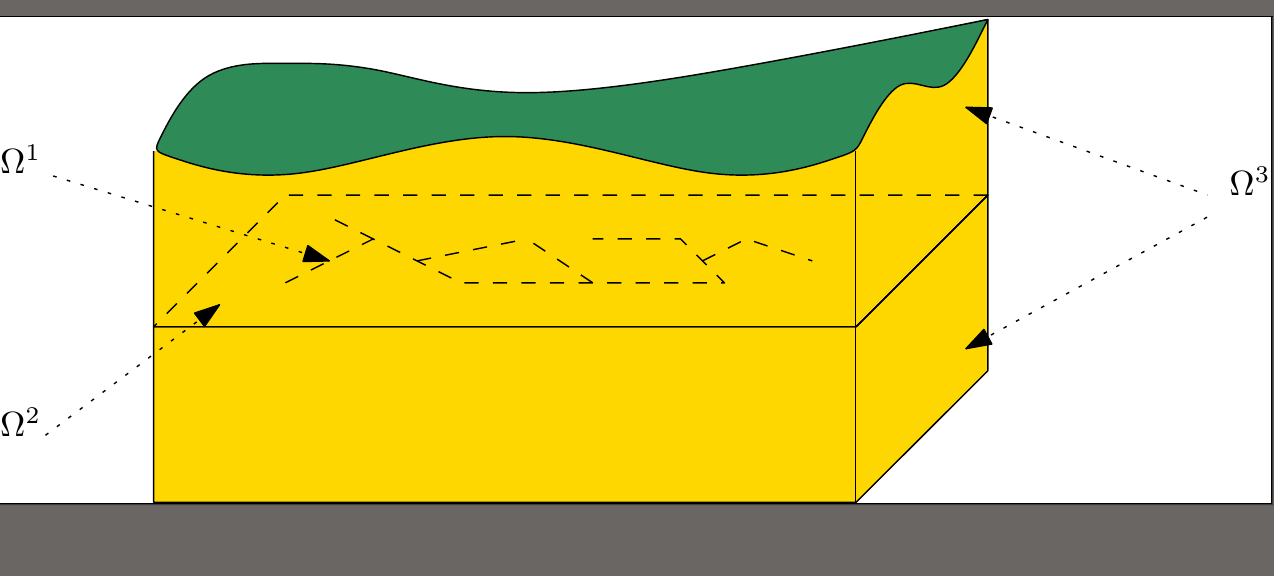
\includegraphics[width=10cm]{ground_fractures}
\end{figure}

\subsection{Physical model}
On the domain $\Omega^d$ of dimension $d\in\{1,2,3\}$, we consider a system of mass balance equations in the following form:
\begin{equation}
    \label{e:ADE}
   \partial_t ( \th c^i) + \div ( \vc q c^i ) - \div (\th \D^i \grad c^i ) = F(c^1,\dots, c^s)  \quad \text{ on } \Omega^d.
\end{equation}
The principal unknown is the concentration $c^i$ $[kg\,m^{-3}]$ of a substance $i\in\{1,\dots, s\}$, which means weight of the substance in unit volume of the water.
Other quantities are:
\begin{itemize}
\item $\th$ $[-]$ is the porosity, i.e. fraction of space occupied by water and the total volume.
\item $\vc q$ $[m\,s^{-1}]$ is the Darcy flux or the \emph{macroscopic} water velocity.
It is related to the \emph{microscopic} water velocity $\vc v$ by the relation $\vc q = \th\vc v$.
\item The hydrodynamic dispersivity tensor $\D^i$ $[m^2 s^{-1}]$ has the form
\[
  \D^i =D_m^i \tau \tn I + \abs{\vc v}\big(\alpha_T^i \tn I + (\alpha_L^i - \alpha_T^i) \big) \frac{\vc v \times \vc v}{\abs{\vc v}^2},
\]
which models (isotropic) molecular diffusion, and dispersion in longitudal and transversal direction to the flow.
Here $D_m^i$ $[m^2\,s^{-1}]$ is the molecular diffusion coefficient of the $i$-th substance (usual magnitude in clear water is $10^{-9}$), $\tau=\th^{1/3}$ is the tortuosity (by \cite{millington_quirk}), $\alpha_L^i$ and $\alpha_T^i$ is the longitudal and the transversal dispersivity $[m]$, respectively.

\item The reaction term $F(\dots)$ is currently neglected.
\end{itemize}


In lower dimensions $d=1,2$, equation \eqref{e:ADE} represents transport processes in planar or channel fractures whose cross-cut $\delta^d$ ($[m]$ for 2D and $[m^2]$ for 1D) is negligible with respect to the dimensions of the physical domain.
For $d=3$ we set $\delta^3=1$ $[-]$.


\paragraph{Boundary conditions.}
The physical boundary $\partial\Omega^d$ is decomposed into two parts:
\begin{align*}
\Gamma_D(t) &= \{\vc x\in \partial\Omega^d\where \vc q(t,\vc x)\cdot\vc n(\vc x)<0\},\\
\Gamma_N(t) &= \{\vc x\in \partial\Omega^d\where \vc q(t,\vc x)\cdot\vc n(\vc x)\ge 0\},
\end{align*}
where $\vc n$ stands for the unit outward normal vector to $\partial\Omega^d$.
On the inflow part $\Gamma_D$, concentrations have to be prescribed (Dirichlet boundary condition):
$$ c^i(t,\vc x) = c^i_D(t,\vc x) \mbox{ on }\Gamma_D(t), $$
while on $\Gamma_N$ we impose homogeneous Neumann boundary condition:
$$ -\D^i(t,\vc x)\nabla c^i(t,\vc x)\cdot\vc n(\vc x) = 0 \mbox{ on }\Gamma_N(t). $$




\paragraph{Communication between dimensions.}
Transport of substances is considered also on interfaces of physical domains with adjacent dimensions (i.e. 3D-2D and 2D-1D, but not 3D-1D).
Denoting $c_{d+1}$, $c_d$ the concentration of a given substance in $\Omega^{d+1}$ and $\Omega^d$, respectively, the comunication on the interface between $\Omega^{d+1}$ and $\Omega^d$ is described by:
\begin{equation}
  \label{e:inter_dim_flux}
  q^c = \sigma^c (c_{d+1} - c_d) + \begin{cases}q^w c_{d+1} & \mbox{ if }q^w\ge 0,\\q^w c_d & \mbox{ if }q^w<0,\end{cases}
\end{equation}
where
\begin{itemize}
\item $q^c$ $[kg\, m^{-2}\,s^{-1}]$ is the concentration flux from $\Omega^{d+1}$ to $\Omega^d$,
\item $\sigma^c$ $[m\,s^{-1}]$ is a transition parameter,
\item $q^w$ $[m\,s^{-1}]$ is the water flux from $\Omega^{d+1}$ to $\Omega^d$.
\end{itemize}
Equation \eqref{e:inter_dim_flux} is incorporated as a boundary condition for the problem on $\Omega^{d+1}$:
$$ -\D\nabla c_{d+1}\cdot\vc n + q^w c_{d+1} = q^c $$
and a source term in $\Omega^d$:
$$ F^c_d = \frac{\delta_{d+1}}{\delta_d}(\sigma^c+\abs{q^w})(c_{d+1}-c_d). $$



\section{Numerical solution}

For the numerical approximation of the advection-diffusion equation \eqref{e:ADE} we distinguish whether diffusion is present or not.
Since the true solution has qualitatively different properties, we also choose different numerical methods for each case.

\subsection{Pure advection}

\subsection{Advection with diffusion}

For the general case we use the discontinuous Galerkin space approximation and implicit Euler time discretization.
Let $\tau$, $h$ be the time step and the space discretization parameter, respectively.
We assume that $\Th^d$ is a regular partition of the domain $\Omega^d$ into simplices, $d=1,2,3$.
We define the set $\Eh^d$ of all edges of elements in $\Th$ (triangles for $d=3$, line segments for $d=2$ and points for $d=1$).
Further, $\Ehint^d$ will denote interior edges, $\Ehdir^d$ edges that coincide with $\Gamma_D^d$ and $\Ehcom^d$ stands for edges on interface with $\Omega^{d-1}$.

Let us fix one substance and the space dimension $d$.
At each time instant we search for the concentration field $c_d^h\in V_d^h$, where
$$ V_d^h = \{v:\overline{\Omega^d}\to\R\where v_{|T}\in P_1(T)~\forall T\in\Th^d\} $$
is the space of functions piecewise affine on the elements of $\Th^d$, possibly discontinuous across the element interfaces.
The discrete problem reads:
$$ \sc{\th\frac{c_d^h-c^h_{d,old}}\tau}{v}_{\Omega^d} + a^h_d(c^h_d,v) = b^h_d(v) \quad \forall v\in V^h_d. $$
Here $c^h_{d,old}$ is the solution from the previous time step and the forms $a^h_d$, $b^h_d$ are defined as follows:
\begin{multline*}
a^h_d(u,v) = \sc{\th\D\nabla u}{\nabla v}_{\Omega^d}
+ \sc{(\div\vc q)u}{v}_{\Omega^d}
+ \sc{\vc q\cdot\nabla u}{v}_{\Omega^d}\\
- \th\sum_{E\in\Ehint^d}\left(\sc{\avg{\D\nabla u}\cdot\n}{\jmp{v}}_E + \sc{\avg{\D\nabla v}\cdot\n}{\jmp{u}}_E\right)\\
- \sum_{E\in\Ehint^d}\sc{\vc q\cdot\n\avg{v}}{\jmp{u}}_E
+ \sum_{E\in\Ehint^d}\gamma_E\sc{\jmp{u}}{\jmp{v}}_E
+ \sum_{E\in\Ehdir^d}\gamma_E\sc{u}{v}_E,
\end{multline*}
% 
\begin{equation*}
b^h_d(v) = \sum_{E\in\Ehdir^d}\gamma_E\sc{c_D}{v}_E.
\end{equation*}
For an interior edge $E$ we denote by $T^-(E)$ and $T^+(E)$ the elements sharing $E$.
By $\n$ we mean the unit normal vector to $E$ pointing from $T^-(E)$ towards $T^+(E)$, the inter-element jump is defined as $\jmp{f}=f_{|T^-(E)}-f_{|T^+(E)}$, and $\avg{f}=\omega f_{|T^-(E)} + (1-\omega) f_{|T^+(E)}$ denotes a weighted average of the quantity $f$.
The weight $\omega$ is chosen in a specific way (see \cite{ern_stephansen_zunino} for details) taking into account possible inhomogeneity of $\D$.
The stabilization parameter $\gamma_E>0$ is user dependent; its value affects the inter-element jumps of the solution.

If there are interfaces between adjacent dimensions, then the following terms are added to the left and right hand side, respectively:
$$ a^h_{d,com}(u,v) = \sum_{E\in\Ehcom^d} (\sigma^c+(q^w)^-)\sc{u}{v}_E - \sum_{T\in\Th^d\cap\Ehcom^{d+1}}(\sigma^c+\abs{q^w})\sc{u}{v}_T, $$
$$ b^h_{d,com}(v) = \sum_{E\in\Ehcom^d} (\sigma^c+(q^w)^-)\sc{c^h_{d-1}}{v}_E - \sum_{T\in\Th^d\cap\Ehcom^{d+1}}(\sigma^c+\abs{q^w})\sc{c^h_{d+1}}{v}_T. $$
Here we obviously set $\Ehcom^4=\Ehcom^1=\emptyset$.

% TODO:
% \begin{itemize}
%   \item Write equations for sorption and integrate them into \eqref{e:ADE}. 
% $R_i(\argdot)$ is a ``retardation function'' its a function which includes various types of equilibrium sorption.
% It is in general dependent as on the substance $i$ as on the material in particular location in space. 
% 
% \end{itemize}
% 
% 
% 
% 
% \begin{enumerate}
%  \item Explicit solution - technicaly this is only slight modification of the already implemented transport model. One has to add appropriate 
%        diffusive flux approximation. Something was done by Sembera nad Jiranek, however there are more possible approximations (further search). Weakness:
%        \begin{itemize}
%         \item too restrictive condition on timestep size for big diffusion on small elements
% 	      \[
% 	         dt \le \min \frac{dx^2}{2D},\qquad dt\le \min \frac{dx}{v}
% 	      \]
% 	\dots so the former condition is more restrictive if $\min dx / D \le 2\min 1/v$ \dots Peclet number can not be used since it 
%         measure only local balnace between diffusion and convection
% 
%         \item persisting problems with CFL condition
%         \item problems with approximation of the diffusive flux with anisothropy raising from the dispersion
%        \end{itemize}
%   \item Implicit solution
%   \begin{enumerate}
%        \item Finite volumes/ Discontinuous Galerkin - search for suitable approximation of the diffusive flux (as above)
%        \item Lumped MH  for diffusion, upwind for convection. Problem with zero or nearly zero $\tn D$. There has to be also implementation without
%              diffusion (no whole MH stuff). Problem that with lumping this leads to edge centered finite volumes.
%   \end{enumerate}   
%   
% \end{enumerate}



\bibliographystyle{abbrvnat}
\bibliography{ref}


\end{document}
